\input{"preamble"}

\usepackage{tabularx}

\hypersetup{
  colorlinks=true,
  linkcolor=black,
  citecolor=black,
  urlcolor=cyan
}

\usepackage[round]{natbib}
\bibliographystyle{plainnat}

\graphicspath{{"./fig/"}}


\def \goml {\href{http://www.ebi.ac.uk/QuickGO/GTerm?id=GO:0051646}{GO:0051646} (mitochondrion localization)}
\def \gomml {\href{http://www.ebi.ac.uk/QuickGO/GTerm?id=GO:0051659}{GO:0051659} (maintenance of mitochondrion localization)}
\def \gomert {\href{http://www.ebi.ac.uk/QuickGO/GTerm?id=GO:1990456}{GO:1990456} (mitochondrion-ER tethering)}
\def \goeml {\href{http://www.ebi.ac.uk/QuickGO/GTerm?id=GO:0051654}{GO:0051654} (establishment of mitochondrion localization)}
\def \gommaaf {\href{http://www.ebi.ac.uk/QuickGO/GTerm?id=GO:0034642}{GO:0034642} (mitochondrial migration along actin filament)}
\def \goemlmm {\href{http://www.ebi.ac.uk/QuickGO/GTerm?id=GO:0034643}{GO:0034643} (establishment of mitochondrial localization, microtubule mediated)}
\def \goemlma {\href{http://www.ebi.ac.uk/QuickGO/GTerm?id=GO:0034640}{GO:0034640} (establishment of mitochondrion localization by microtubule attachment)}
\def \gomtam {\href{http://www.ebi.ac.uk/QuickGO/GTerm?id=GO:0047497}{GO:0047497} (mitochondrion transport along microtubule) }
\def \goemlimf {\href{http://www.ebi.ac.uk/QuickGO/GTerm?id=GO:0090146}{GO:0090146} (establishment of mitochondrial localization involved in mitochondrial fission)}
\def \goremlimf {\href{http://www.ebi.ac.uk/QuickGO/GTerm?id=GO:0090147}{GO:0090147} (regulation of establishment of mitochondrion localization involved in mitochondrial fission)}
\def \gomd {\href{http://www.ebi.ac.uk/QuickGO/GTerm?id=GO:0048311}{GO:0048311} (mitochondrion distribution)}
\def \goidm {\href{http://www.ebi.ac.uk/QuickGO/GTerm?id=GO:0048312}{GO:0048312} (intracellular distribution of mitochondria)}
\def \gomi {\href{http://www.ebi.ac.uk/QuickGO/GTerm?id=GO:0000001}{GO:0000001} (mitochondrion inheritance)}

\def \SyRO {\href{https://github.com/hyginn/SyRO}{github.com/hyginn/SyRO}}
\def \firstpool {\href{https://github.com/thejmazz/biologicalsystem/blob/master/notebook.md\#user-content-summary-of-first-pool}{notebook}}

\newcommand{\uniprot}[1]{\href{http://www.uniprot.org/uniprot/#1}{#1}}

\begin{document}

\title{
\vspace{-155pt}
\hspace*{-80pt}\includegraphics[width=1.35\linewidth]{"purkinje-neuron-mitochondria"}
Neuronal Mitochondrion Trafficking \\
\small{\textit{BCH441 Project: Defining a System}}
}
\author{Julian Mazzitelli}
\date{\today}

\maketitle

\begin{bottompar}
\begin{center}
\textit{
The source code, notebook, and data pipeline can be found at
\href{https://github.com/thejmazz/biologicalsystem}{github.com/thejmazz/biologicalsystem}. \\
Cover image (mitochondrion in Purkinje neuron) by Atlas of Ultrastructural Neurocytology\footnote{\href{http://synapses.clm.utexas.edu/atlas/1_1_2_8.stm}{synapses.clm.utexas.edu/atlas/1\_1\_2\_8.stm}}
}
\end{center}
\end{bottompar}

\tableofcontents


\section{Introduction}

The ``powerhouse of the cell'' as it is so commonly called, the mitochondria is
one of the most vital organelles in eukaryotes. This structure is thought to
have developed through a symbiotic relationship among engulfed prokaryotic cells
and their hosts. As such, it is rooted quite deeply evolutionarily, and one
might expect its proper functioning to be absolutely vital, that is, knock-out
mutants will not survive. This is true - but as we will see, it is not just the
performance of this organelle which is centrally important, but where it is
localized within the cell as well.

Images of isolated mitochondria were first observed in \citeyear{Lincoln1979}
by \citeauthor{Lincoln1979}:

\begin{center}
  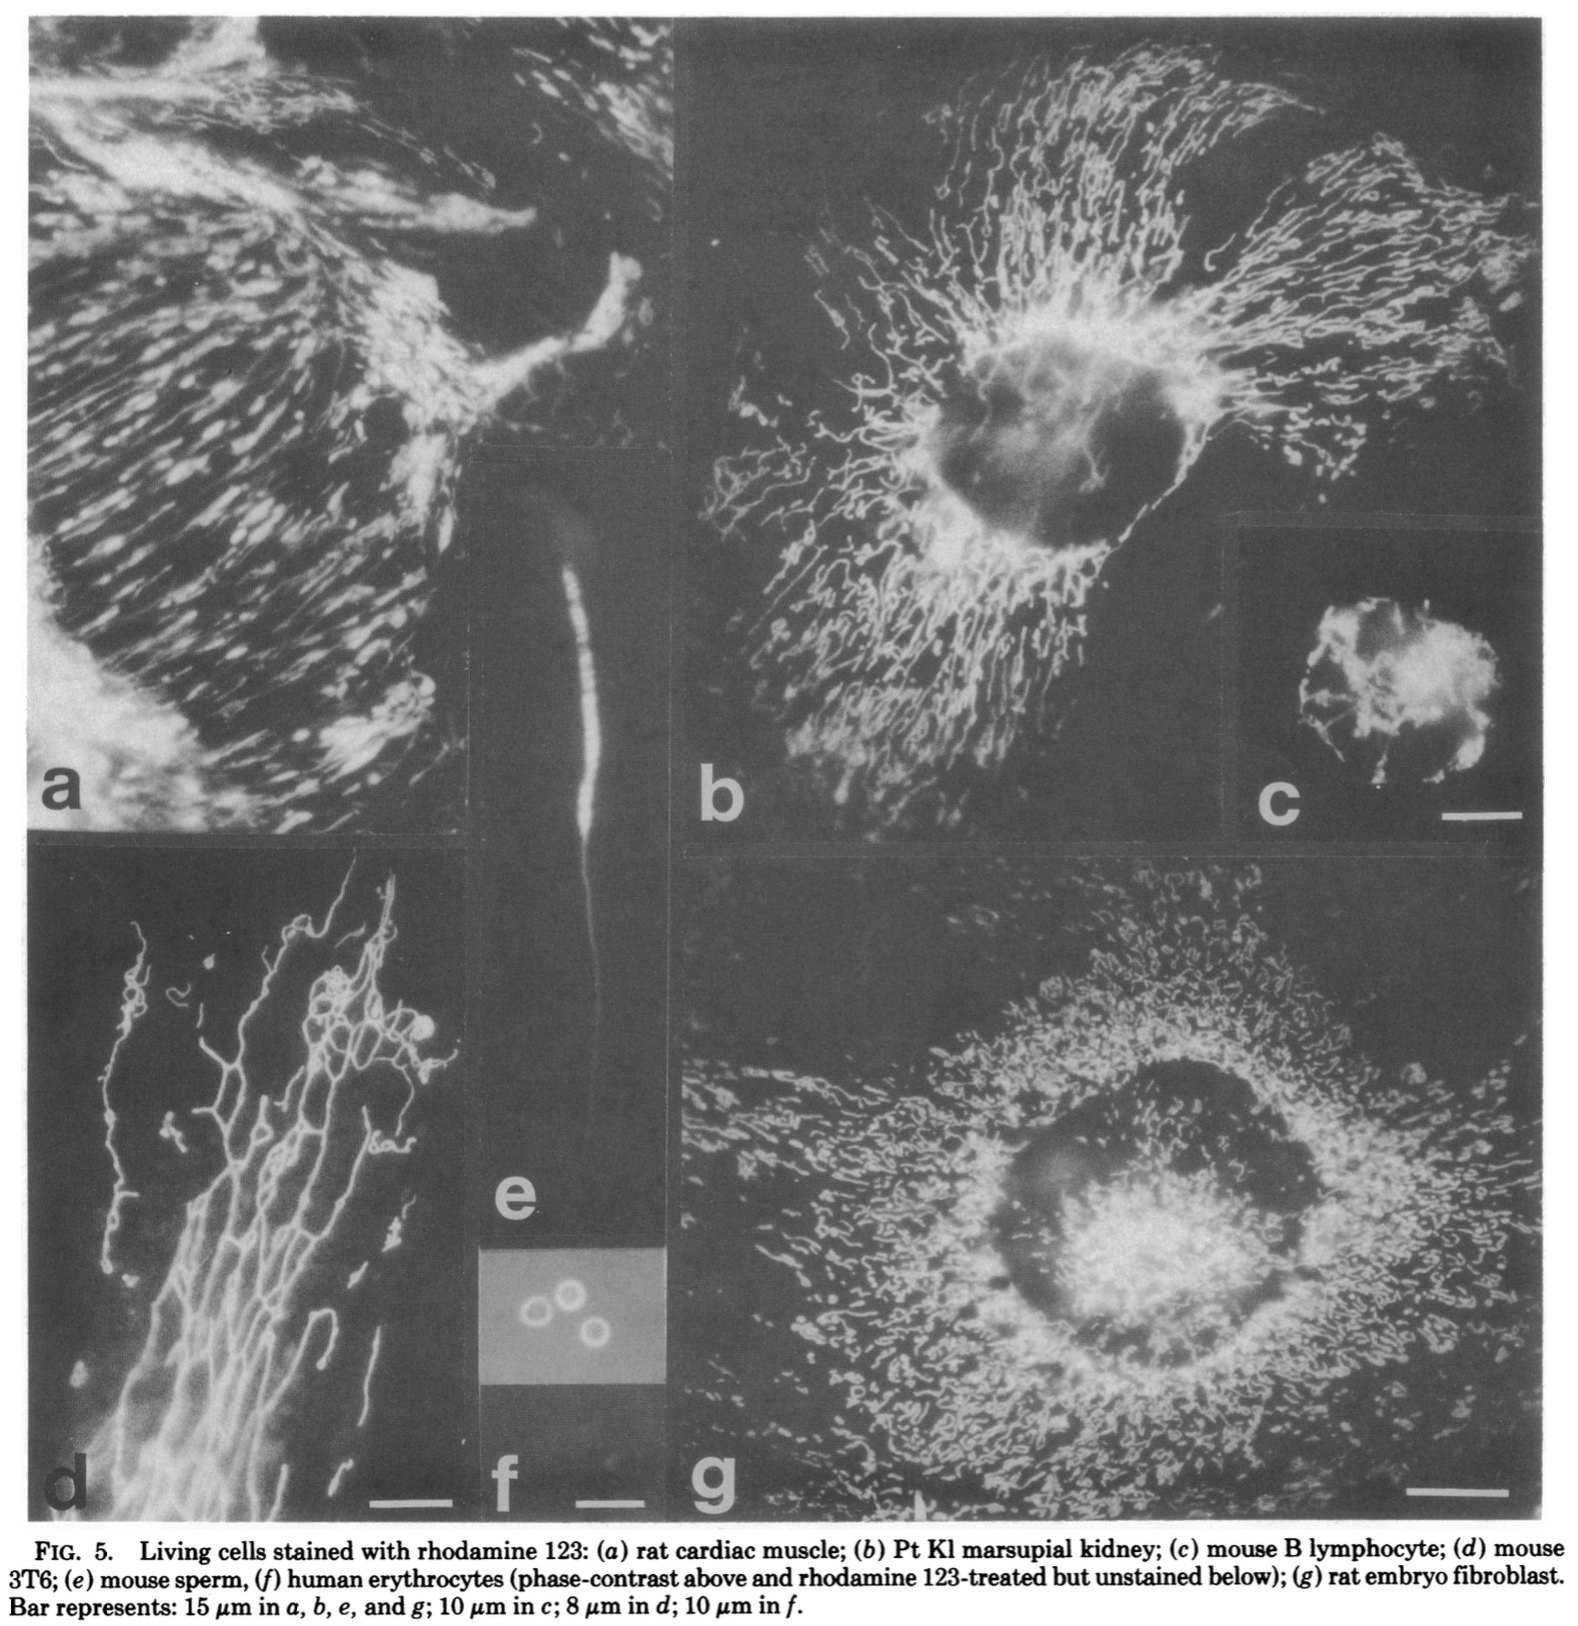
\includegraphics[width=0.6\linewidth]{rhodamine-mitochondria}
\end{center}

\noindent The variety of mitochondrion shape and size is clear, ranging from
globular to filamentous to networked structures. As well, the authors observed
movement during 15-30 sec intervals, between fluorescent and phase-contrast
photographs.

The primary role of a mitochondrion is to supply energy to the cell in the form
of ATP units, through the electron transport chain among the cristae. Where is
that energy needed? Consider highly polar and elongated cells such as neurons.
The cell body of a neuron is distant from its synaptic endings, where as it
happens, large amounts of energy are required for neurotransmitter release and
absorption. Following, we will investigate the \textbf{system} whose
\textbf{functional role} is the \textbf{localization of mitochondrion within
neurons}.

\section{The System}

\begin{tabularx}{\linewidth}{l X}
  \textit{Name} & Localization/Trafficking of mitochondrion within neurons \\
  \textit{Description} & The collective of functional units represented by genes which process signals, transduce these events, initiate, and maintain the actions necessary to transport mitochondrion to distal points along the axon of a neuron. \\
  \textit{Associated GO Terms} & \goml
\end{tabularx}

\begin{itemize}
  \item \gomml
  \begin{itemize}
    \item \gomert
  \end{itemize}
  \item \goemlmm
  \begin{itemize}
    \item \gommaaf
    \item \goemlmm
    \begin{itemize}
      \item \goemlma
      \item \gomtam
    \end{itemize}
    \item \goemlimf
    \begin{itemize}
      \item \goremlimf
    \end{itemize}
  \end{itemize}
  \item \gomd
  \begin{itemize}
    \item \goidm
    \item \gomi
  \end{itemize}
\end{itemize}

Why this system? Originally I was looking into ``mitochondrial localization.''
Amongst the genes returned by the ontology, there appeared those related to
mitochondrial localization during cellular reproduction, transport,
microtubules, tethers, mRNA-binding, and various ``popular'' genes such as
ubiqutins, serum  albumin, leucine-rich repeat serine/threonine-protein kinase,
basic helix-loop-helix protein. There was a fair amount of variety. In order to
gather together a structured list of genes I would need to filter these out, and
to filter these out I would need a functional goal. I decided to choose the
neuronal process because it is one of the most extreme cases of mitochondrial
movement in all cell types, there was a decent amount of related literature
available, some elements of its processes had been recently elecidated, and it
has important neurophysiological consequences. A review by \cite{Reis2009}
explored the atypical Miro GTPases and their role in transporting mitochondria
in neurons. The authors note that abnormal mitochondrial dynamics can contribute
to Amyotropic Lateral Sclerosis (ALS), Huntington's, Parkinson's, and
Alzheimer's diseases. A more recent experiment by \cite{Loss2015} examines the
role of TRAK1 and TRAK2 kinesin adaptor proteins which link mitochondria to
kinesin motor proteins. Furthermore, Miro proeins are expressed in a large
variety of cell types, potentially extending this current analysis to new
domains \citep{Reis2009}.

\subsection{Systems Role Ontology}

To define this system in a structured manner, I considered its functionality
in the context of the Systems Roles Ontology, which can be found at \SyRO:

\begin{center}
  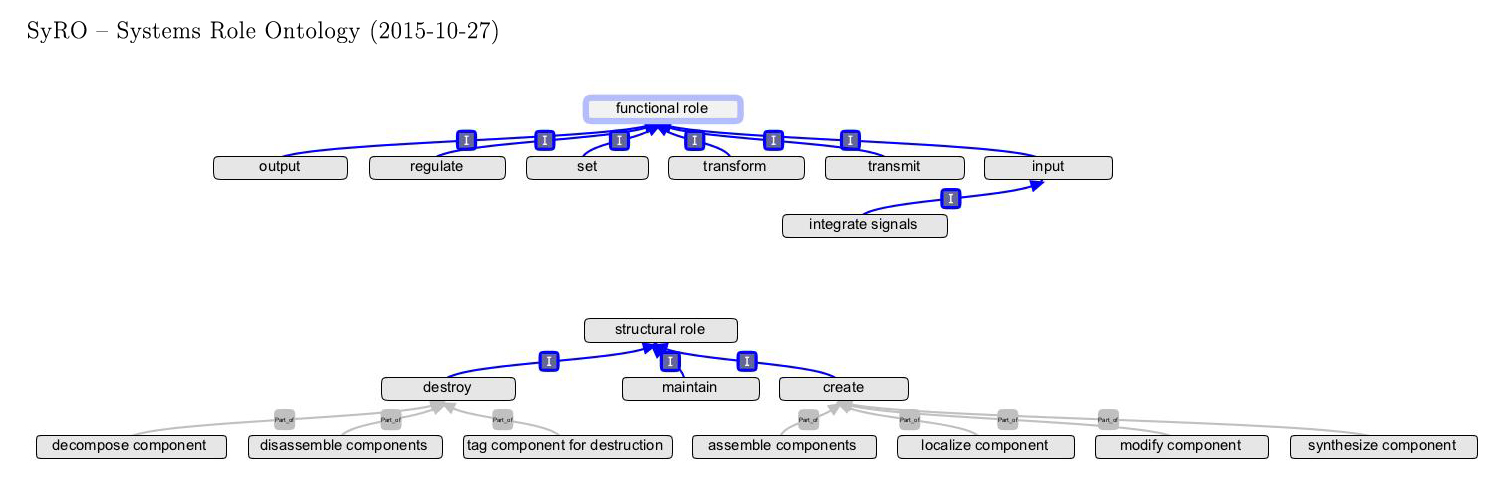
\includegraphics[width=1\linewidth]{SyRO-2015-10-27}
\end{center}

\begin{tabularx}{\linewidth}{l l X}
  \textit{\textcolor{grey}{Name}} & \textit{\textcolor{grey}{ID}} & \textit{\textcolor{grey}{Context Within Neuronal Mitochondrion Localization}} \\
  \textbf{input} & \texttt{16} & compounds or signals prompting the directed movement of mitochondrion \\
  \textbf{integrate signals} & \texttt{22} & machinery which directs input signals/compounds to the system \\
  \textbf{output} & \texttt{21} & mitocondrion transport towards synaptic endings \\
  \textbf{regulate} & \texttt{20} & components which ensure regular mitochondrial motility \\
  \textbf{set} & \texttt{19} & preparing the functional units, ``setting the stage'' as it were  \\
  \textbf{transform} & \texttt{18} & altering the system status so that it may be reversed, stopped, reinstated \\
  \textbf{transmit} & \texttt{17} & the physical machinery to move mitochondria \\
\end{tabularx} \\

These functions collaborate to produce the \textbf{functional role} of
localizing mitochondria \textbf{for the proper functioning of neural
communication}. I will define the bounds of this system as any genes which can
be annotated with the functional role annotations above. Structural role
annotations will be considered second to function, and will be used largely to
describe how that component physically determines its function. With this goal
in mind, I fetched and filtered data from the Gene Ontology Consortium, QuickGO,
UNIPROT, IntAct, and STRING. Those genes which did not make the cut can be seen
through the \textit{Summary of first pool} in my \firstpool.

\section{Gene Collection}

\rowcolors{2}{white}{gray!25}
\begin{tabularx}{\linewidth}{l l l X}
  \textit{Gene} & \textit{Accession} & \textit{Name} & \textit{SyRO} \\
  ATCAY & \uniprot{Q86WG3} & Caytaxin & regulate \\
  BHLHA15 & \uniprot{Q7RTS1} & Class A basic helix-loop-helix protein 15 & transmit \\
  CLUH & \uniprot{I3L2B0} & Clustered mitochondria protein homolog & set \\
  GABA & \uniprot{P80404} & Gamma-amino-N-butyrate transaminase & transmit \\
  GAN & \uniprot{Q9H2C0} & Gigaxonin & transform \\
  KIF1B & \uniprot{O60333} & Kinesin-like protein KIF1B & output \\
  KIF5B & \uniprot{P33176} & Kinesin-1 heavy chain & output \\
  KLCA1 & \uniprot{Q07866} & Kinesin light chain 1 & output \\
  MAPT & \uniprot{P10636} & Microtubule-associated protein tau & set \\
  MAP1B & \uniprot{P46821} & Microtubule-associated protein 1B & set \\
  MGARP & \uniprot{Q8TDB4} & Mitochondria-localized glutamic acid-rich protein & regulate \\
  MTM1 & \uniprot{Q13496} & Myotubularin & set \\
  MSTO1 & \uniprot{Q9BUK6} & Protein misato homolog 1 & regulate \\
  RHOT1 & \uniprot{Q8IXI2} & Mitochondrial Rho GTPase 1 & integrate signals \\
  RHOT2 & \uniprot{Q8IXI1} & Mitochondrial Rho GTPase 2 & integrate signals \\
  SNPH & \uniprot{O15079} & Syntaphilin & regulate \\
  SYBU & \uniprot{Q9NX95} & Syntabulin & set \\
  TIAM2 & \uniprot{Q8IVF5} & T-lymphoma invasion and metastasis-inducing protein 2 & integrate signals \\
  TRAK1 & \uniprot{Q9UPV9} & Trafficking kinesin-binding protein 1 & transmit \\
  TRAK2 & \uniprot{Q8IU62} & Trafficking kinesin-binding protein 2 & transmit \\
  TTL & \uniprot{Q8NG68} & Tubulin--tyrosine ligase & transform \\
\end{tabularx}

\section{Documentation}

\subsection{Signal Integration}

\subsubsection{RHOT1, RHOT2 \textit{Mitochondrial Rho GTPase 1, 2}}

RHOT1 and RHOT2, which are also known as MIRO1 and MIRO2, were first reported as
a new family of Rho GTPases with in \citeyear{Fransson2003} by
\citeauthor{Fransson2003}. An NCBI CDD search presents us with two GTPase
domains at each terminus, with two EF hands in between. The C terminal TM domain
targets this protein to the mitochondria.

\begin{figure}[h]
  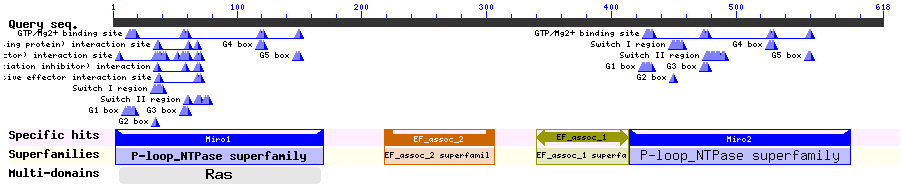
\includegraphics[width=1.0\linewidth]{Rhot-CDD}
\end{figure}

NTPases are a large superfamily and operate in a large variety of systems. The
on/off state of these proteins confers their ability to integrate signals into a
pathway. In this way we can observe that whichever is activiting Rhot, Rhot is
integrating that signal downwards to its effector. \citeauthor{Fransson2003}
also observed an interesting property: overexpression of Miro1/Val-13 led to
an aggregation of the mitochondrial network. The same authors separated this
response into two distinct phenotypes later in \citeyear{Fransson2006}. They
observed that Miro-1 induced aggregration and thread-like mitochondria, whereas
Miro-2 only induced aggregation. \citeauthor{Fransson2006} also demonstrated
interactions of Miro with GRIF-1 (TRAK2) and OIP106 (TRAK1), trafficking
kinesin binding proteins. The EF hands can bind calcium,
disrupting interactions with TRAK \citep{Reis2009}.

% Ability to bind to TRAK1 not Ca2+ dep.

% TODO move to regulation?
\subsubsection{TIAM2 \textit{T-lymphoma invasion and metastasis-inducing protein 2}}

TIAM2 regulates the activity of RHO-like proteins (UNIPROT). This is confirmed
with the existence of a GEF domain from the CDD.

\begin{figure}[h]
  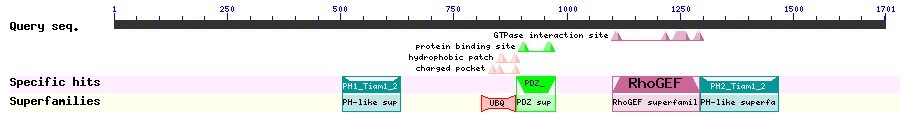
\includegraphics[width=1.0\linewidth]{TIAM2-CDD}
\end{figure}

In this way TIAM2 has the ability to activate Rhot. TIAM2 has also been shown to
promote the migration of neurons in the cerebral cortex (UNIPROT).

\subsection{Set}

\subsubsection{CLUH \textit{Clustered mitochondria protein homolog}}

A CDD search with CLU1 from yeast presents the CLU domain (CLUstered
mitochondria). This domain is required for mitochondrial positioning and
transport; improper function can lead to mitochondrion clustering at the
microtubule plus ends (CDD). Another uncharactized CLU domain is present.

\begin{center}
  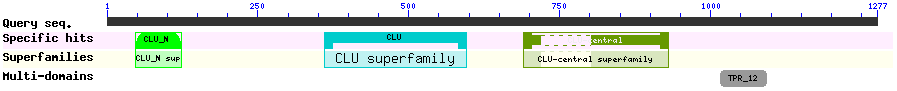
\includegraphics[width=1.0\linewidth]{CLU1-CDD}
\end{center}

\subsubsection{MAP1B \textit{Microtubule-associated protein 1B}}

By similarity, MAP1B facilitates tyrosination of $\alpha$-tubulin in
neuronal microtubules. Interacts with TIAM2 and TTL (UNIPROT). IntAct
suggests an interaction with GAN.

\begin{center}
  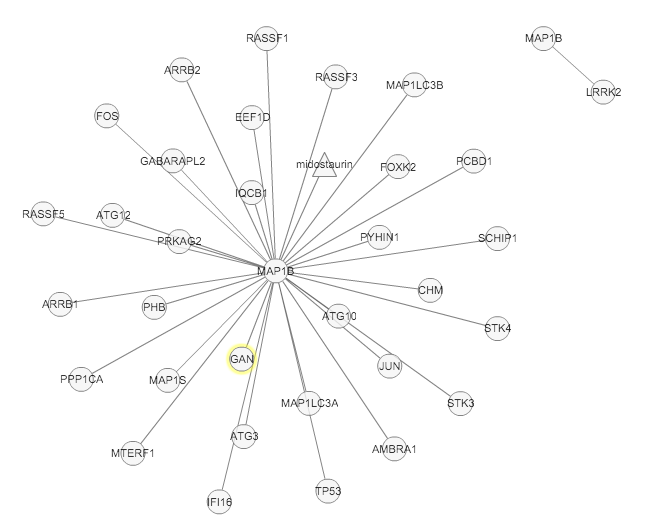
\includegraphics[width=0.5\linewidth]{MAP1B-IntAct}
\end{center}

\subsubsection{MAPT \textit{Microtubule-associated protein tau}}

CDD for MAPT presents tubulin binding repeat domains. MAPT is expected to
stablize microtubules and potentially establish and maintain neuronal polarity
(UNIPROT).

\begin{center}
  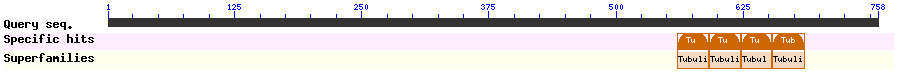
\includegraphics[width=1.0\linewidth]{MAPT-CDD}
\end{center}

\subsubsection{MTM1 \textit{Myotubularin}}

\cite{Hnia2011} observed that decreased MTM1 expression and mutations
induced abnormal mitochondrial positioning, shape, dynamics, and function.

\subsubsection{SYBU \textit{Syntabulin}}

SYBU belongs to a kinesin motor-adapter complex. It is critical for forward
axonal transport (UNIPROT). STRING demonstrates binding interactions with
KIF5B, which in turn binds with KIF5A and TRAK2, of which both bind TRAK1.

\begin{center}
  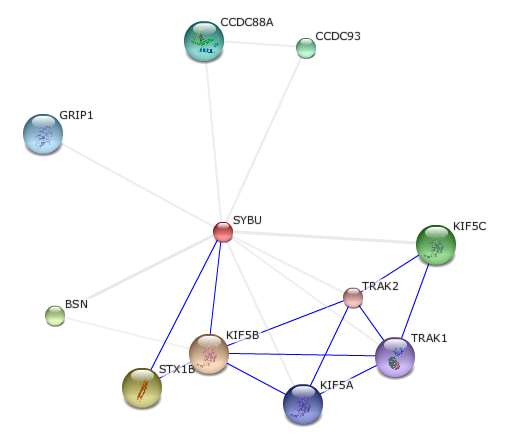
\includegraphics[width=0.5\linewidth]{SYBU-STRING}
\end{center}

\cite{Reis2009} note that syntabulin has been found to interact with kinesin
heavy chain in hippocampal neurons.

\subsection{Transmit}

\subsubsection{BHLHA15 \textit{Class A basic helix-loop-helix protein 15}}

Required for mitochondrial calcium ion transport (UNIPROT). Ensembl electronic
annotation has tagged BHLHA15 with the biological process
\href{http://www.ebi.ac.uk/QuickGO/GTerm?id=GO:0019722}{calcium-mediated
signalling}. This protein is expressed specifically in brain, liver,
spleen and skeletal muscle (UNIPROT).

\subsubsection{GABA \textit{Gamma-amino-N-butyrate transaminase}}

GABA is located within the mitochondrial matrix (UNIPROT). Does not appear
particularly involved on its own, yet we will see it interacts with TRAK1 and
TRAK2.

\subsubsection{TRAK1, TRAK2 \textit{Trafficking kinesin-binding protein 1, 2}}

\cite{Reis2009} identify Milton as an adapter protein required for the
transport of mitochondria in axons.  The closest human equivalents are TRAK1
and TRAK2, which each contain a coiled-coiled domain. Below are the TRAK1 and
TRAK2 CDD results.

\begin{center}
  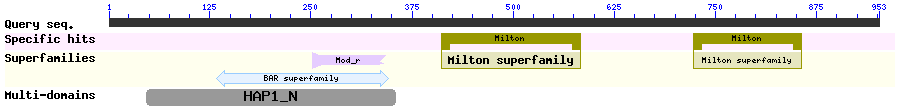
\includegraphics[width=1.0\linewidth]{TRAK1-CDD}
  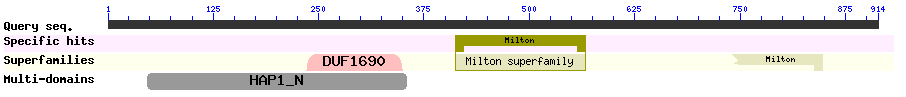
\includegraphics[width=1.0\linewidth]{TRAK2-CDD}
\end{center}

The Milton domain is credited for recruitment of kinesin heavy chain to the
mitochondria (CDD). TRAK1 and TRAK2 have demonstrated interactions with
GABA receptors \citep{Resi2009}. It was previously noted that GABA is located
within the mitochondrion and mitochondrial matrix. UNIPROT mentions TRAK is
involved in the regulation of trafficking GABA receptors.

STRING corroborates with interactions for SYBU above. As well make note of the
identified binding between TRAK2, MGARP and RHOT1.

\begin{center}
  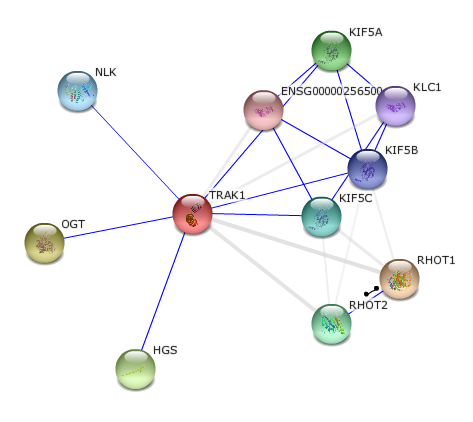
\includegraphics[width=0.45\linewidth]{TRAK1-STRING}
  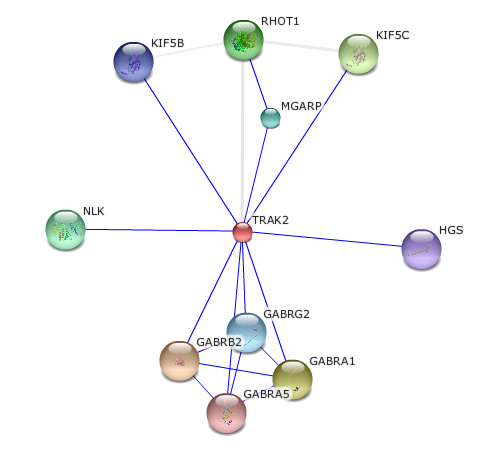
\includegraphics[width=0.45\linewidth]{TRAK2-STRING}
\end{center}

\subsection{Transform}

\subsubsection{GAN \textit{Gigaxonin}}

\cite{Allen2005} observed that GAN interacts with the light chain of MAP1B.
IntAct also suggests this interaction.

\begin{center}
  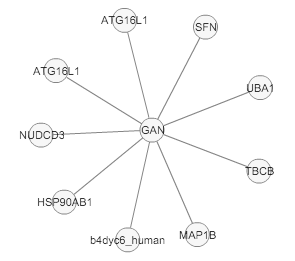
\includegraphics[width=0.25\linewidth]{GAN-IntAct}
\end{center}

When \citeauthor{Allen2005} deleted sequences for binding to GAN from MAP1B,
the N terminus of MAP1B was not ubiquitinated. This suggests that GAN plays
a regulatory role with MAP1B, and since MAP1B facilitates forward movement
of mitochondria along microtubules, GAN has the potential to arrest this
process.

\subsubsection{TTL \textit{Tubulin--tyrosine ligase}}

ATP + detyrosinated $\alpha$-tubulin + L-tyrosine = $\alpha$-tubulin + ADP +
phosphate (UNIPROT). TTL is involved in microtubule organization, given its
modifications to $\alpha$-tubulin, a primary component of microtubules.

\subsection{Regulate}

\subsubsection{ATCAY \textit{Caytaxin}}

Has been annotated with \href{http://www.ebi.ac.uk/QuickGO/GTerm?id=GO:0019894}{kinesin binding}
GO molecular function (UniProtKB, inferred from physical interaction).
UNIPROT suggests it may regulate the localization of mitochondria within
axons and dendrites. A CDD search presents the SEC14p-like lipid binding
domain, found in lipid regulated proteins such as RhoGAPs and RhoGEFs.

\begin{center}
  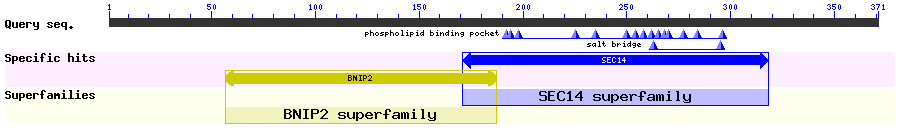
\includegraphics[width=1.0\linewidth]{ATCAY-CDD}
\end{center}

In this way it is possible ATCAY may perform a similar function to TIAM2.

\subsubsection{MGARP \textit{Mitochondria-localized glutamic acid-rich protein}}

MGARP is annoted as an
\href{http://www.ebi.ac.uk/QuickGO/GTerm?id=GO:0031307}{integral component of
mitochondrial outer membrane}, inferred by sequence or structural similarity by
UniProtKB. By STRING we can see that it binds with RHOT1 and TRAK2.

\begin{center}
  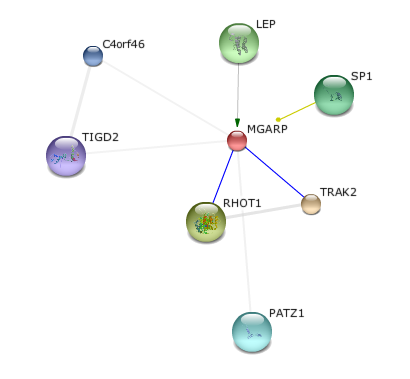
\includegraphics[width=0.35\linewidth]{MGARP-STRING}
\end{center}

The CDD describes a ``mitochondrion localization sequence" as well, supporting
its description as a component of the mitochondrial outer membrane.

\begin{center}
  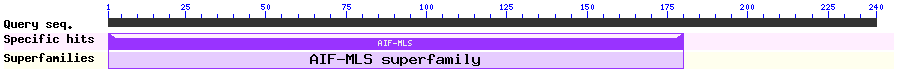
\includegraphics[width=1.0\linewidth]{MGARP-CDD}
\end{center}

It is suggested, by similarity, to translocate TRAK2 from cytoplasm to
mitochondrion (UNIPROT). In this way, we see that RHOT1, RHOT2, TRAK1, TRAK2 and
MGARP all localize at the mitochondrion.

\subsubsection{MSTO1 \textit{Protein misato homolog 1}}

Misato localizes to the outer membrane of mitochondria. It contains a tubulin
like domain and is responsible for mitochondrial fission and localization (CDD).

\begin{center}
  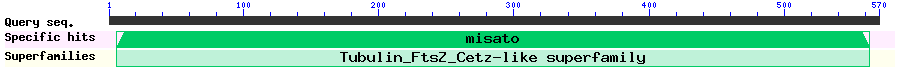
\includegraphics[width=1.0\linewidth]{MSTO1-CDD}
\end{center}

\subsubsection{SNPH \textit{Syntaphilin}}

Syntaphilin is brain specific and found in synapses (UNIPROT). Syntaphilin
has been found co-localized with mitochondria, where it has been proposed
to act as receptor for docking for mitochondria in axons. Furthermore, deletion
of the SNPH gene has resulted in increased mitochondrial motility and reduced
mitochondrial density in axons \citep{Reis2009}.

\subsection{Output}

\subsubsection{KIF1B, KIF5B, KLC1 \textit{Kinesin-like protein KIF1B, heavy chain, light chain}}

Kinesin activity is the final output of these system. We have seen KIF1B, KIF5B
interact with TRAK1 through binding interactions. Kinesin-like protein KIF1B,
kinesin heavy chain, and kinesin light chain will carry mitochondria towards
the plus end of the microtubule. Due to microtubule arrangement in the cell
handled by other processes, this will be towards the synapses, away from the
cell body.

\section{Data Pipeline}

For this project, I implemented a data pipeline using
\href{http://dat-data.com}{dat} and
\href{https://github.com/datproject/gasket}{gasket}. I wrote a small module
which wraps the QuickGO REST API and provides responses in \texttt{Promise} and
\texttt{Stream} format:
\href{https://github.com/thejmazz/bionode-quickgo}{github.com/thejmazz/bionode-quickgo}.
I plan on submitting this to the bionode project and publishing on npm. The CLI
for bionode-quickgo was used in my gasket pipeline:

\inputminted[fontsize=\small]{json}{"../gasket.json"}

This pipeline will take a GO ID, get its annotation from QuickGO in the
specified format, get the Uniprot XML for each protein, bundle all of these into
one object separated into arrays by gene name, sort by number of proteins per
gene, and then output a neatly formatted markdown file complete with links to
Uniprot. I found this essential in getting an idea of the proteins
representative of each GO term. Data is intermediately stored in the version
controlled file storage program dat. Currently, this pipeline requires manual
editing to perform on a new GO term. With a modern text editor this can be done
quickly for all occurences, yet it is not satisfactory. I had begun writing
\href{https://github.com/thejmazz/bionode-obo}{github.com/thejmazz/bionode-obo},
a streaming OBO 1.2 parser, but could not complete it in time. I would've liked
to specify a GO term, and have the above pipeline run for each child term,
recursively. It would be interesting to implement a web interface composed of
``nodes'' and ``pipes'' to interface with biological databases and file types,
much like how complex shaders (see: \href{http://imgur.com/a/CQUIL}{Procudural
Material Monkeys}) are created in programs like Blender.

\bibliography{biblio}


\end{document}
